% @Author: AnthonyKenny98
% @Date:   2020-02-26 09:00:23
% @Last Modified by:   AnthonyKenny98
% @Last Modified time: 2020-03-01 16:24:05

\section{Reduced Instruction Set Computer Background}
    
    \subsection{Instruction Set Architecture}
        \todo[inline, caption={RISC ISA Background}]{Provide a background into ISAs and how they are defined}

    \subsection{RISC Processor Design}
        \todo[inline, caption={RISC Processor Design Background}]{Provide a background into how RISC processors function}

\section{RISC-V ISA}
    \subsection{RV32I}
        \todo[inline,caption={RV32I Background}]{Should include overview of instrucitons, instruction format, register file. Essentially a summary of the relevant sections of the RISC V Manual Volume 1}

    \subsection{Motion Planning Extension}
        \todo[inline, caption={Motion Planning Extension}]{Full description of design of Non standard extension for motion planning. Should follow define, design, build, measure, analyse etc format.}

\section{PhilosophyV}
    \textit{Philosophy IV}, written in 1903 by Mr. Owen Wister of the Class of 1882, recounts the antics of two Harvard students and their last minute attempts to study (or avoid studying) for an exam for which they are hopelessly unprepared. Similarly, this section details the process of my attempt to build a RISC-V processor, by far the most complex part of this Thesis, and a task for which I am unsure of my preparedness. As such, this processor is named Philosphy V; both in reference to the RISC-V ISA for which it is designed, and to the fact that my current situation seems much like a sequel to Mr. Wister's novel.

    \subsection{Baseline Implementation}
        \todo[inline]{Description of Baseline Philosophy V core}
        Figure \ref{fig:philv-core} provides a schematic of the PhilosophyV processor.
        \todo[inline]{Display bigger version of processor.}
        % \newpage
        % \thispagestyle{empty}
        % @Author: AnthonyKenny98
% @Date:   2020-03-01 15:57:31
% @Last Modified by:   AnthonyKenny98
% @Last Modified time: 2020-04-10 06:41:53
\begin{figure}[H]
\begin{centering}
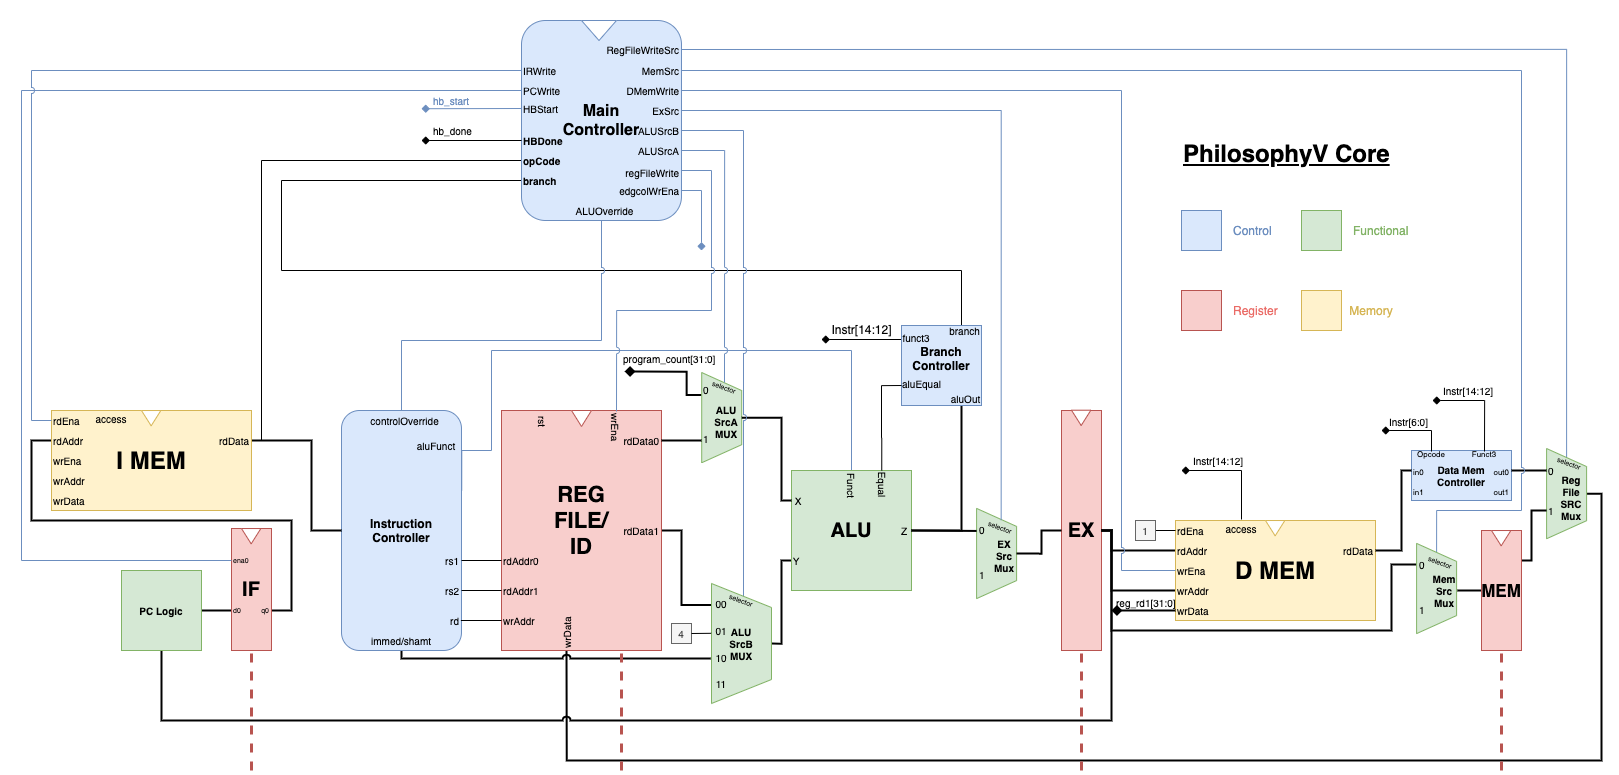
\includegraphics[width=0.7\linewidth]{chapters/chapter4/img/philv-core.png}
\mycaption{RV32I PhilosophyV Schematic}{}
\label{fig:philv-core}
\end{centering}
\end{figure}
 

    \subsection{Implementing HoneyBee}
        \todo[inline]{Process of implementing honeybee into PhilV.}

\section{Performance Analysis}
    \todo[inline]{Comparative Performance Analysis of baseline and extended PhilV Core}